\documentclass{beamer}

\mode<presentation>
{
	\usetheme{CambridgeUS}
	\usecolortheme{orchid}
	\setbeamercovered{transparent}
	\useinnertheme{rectangles}
	\setbeamertemplate{navigation symbols}{}
	\usefonttheme[onlymath]{serif}
	\setbeamercolor{title}{bg=alerted text.fg!85!black, fg=white}
	\setbeamercolor{item projected}{bg=alerted text.fg!85!black}
	\setbeamertemplate{enumerate items}[default]
	\setbeamercolor{local structure}{fg=alerted text.fg!85!black}
}

\usepackage[english]{babel}
\usepackage[utf8]{inputenc}
\usepackage[T1]{fontenc}
\usepackage{lmodern}
\usepackage{pifont}
\usepackage{mathrsfs}
\usepackage{amsmath}
\usepackage{bm}
\usepackage{caption}
\usepackage{subcaption}
\usepackage{outlines}
\usepackage{booktabs}
\usepackage[%
	autocite     = plain,
	doi          = true,
	url          = true,
	giveninits   = true,
	hyperref     = true,
	backref      = true,
	maxbibnames  = 99,
	maxcitenames = 99,
	sortcites    = true,
	style        = authoryear,
]{biblatex}


% \input{bibliography-mimosis}
\addbibresource{presentation.bib}

\newcommand{\fakeimage}{{\fboxsep=-\fboxrule\fbox{\rule{0pt}{3cm}\hspace{4cm}}}}

\usepackage{tikz}
\usetikzlibrary{quotes}
\usetikzlibrary{bayesnet}
\usetikzlibrary{arrows,calc,positioning,decorations.pathreplacing}
\tikzset{
	>=stealth',
	punkt/.style={
			circle,
			draw=black, thick,
			minimum height=1.75em,
			inner sep=0pt,
			text centered},
	pil/.style={
			->,
			thick}
}
\definecolor{hdblue}{HTML}{3366cc}
\hypersetup{colorlinks,linkcolor=,urlcolor=hdblue, citecolor=hdblue}


\newcommand{\xmark}{\ding{55}}
\newcommand{\highlight}[1]{%
	\colorbox{red!50}{$\displaystyle#1$}}


\def\ci{\perp\!\!\!\perp}
\makeatletter
\newcommand*{\indep}{%
	\mathbin{%
		\mathpalette{\@indep}{}%
	}%
}
\newcommand*{\nindep}{%
	\mathbin{%                   % The final symbol is a binary math operator
		\mathpalette{\@indep}{\not}% \mathpalette helps for the adaptation
		% of the symbol to the different math styles.
	}%
}
\def\layersep{.38cm}
\def\inlsep{.4}
\newcommand*{\@indep}[2]{%
	% #1: math style
	% #2: empty or \not
	\sbox0{$#1\perp\m@th$}%        box 0 contains \perp symbol
	\sbox2{$#1=$}%                 box 2 for the height of =
	\sbox4{$#1\vcenter{}$}%        box 4 for the height of the math axis
	\rlap{\copy0}%                 first \perp
	\dimen@=\dimexpr\ht2-\ht4-.2pt\relax
	% The equals symbol is centered around the math axis.
	% The following equations are used to calculate the
	% right shift of the second \perp:
	% [1] ht(equals) - ht(math_axis) = line_width + 0.5 gap
	% [2] right_shift(second_perp) = line_width + gap
	% The line width is approximated by the default line width of 0.4pt
	\kern\dimen@
	{#2}%
	% {\not} in case of \nindep;
	% the braces convert the relational symbol \not to an ordinary
	% math object without additional horizontal spacing.
	\kern\dimen@
	\copy0 %                       second \perp
}
\makeatother


\title[DLBR]{A New Approach to Batch Effect Removal Based on Distribution Matching in Latent Space}

% \subtitle
% {Presentation Subtitle} % (optional)

\author[Dogan]
{%
	\texorpdfstring{
		\begin{columns}
			\column{.85\linewidth}
			\centering
			Huaqing Li, Haluk Dogan, and Juan Cui$^{*}$
		\end{columns}
	}
	{Dogan}
}
\institute[UNL] % (optional, but mostly needed)
{
  Systems Biology and Biomedical Informatics Laboratory\\
  \url{https://sbbi.unl.edu/}\\\vspace{1cm}
  Department of Computer Science and Engineering\\
  University of Nebraska-Lincoln
}

\date[\today] % (optional)
{\today}

\subject{Talks}

\pgfdeclareimage[height=0.5cm]{university-logo}{figures/logo}
\logo{\pgfuseimage{university-logo}}


%\tikzset{every picture/.style={line width=0.75pt}}

\begin{document}

\begin{frame}
  \titlepage{}
\end{frame}

\section{Introduction}
\begin{frame}{Introduction}
  \begin{columns}
	\begin{column}{.55\textwidth}
	  \begin{figure}[ht]
		\centering
		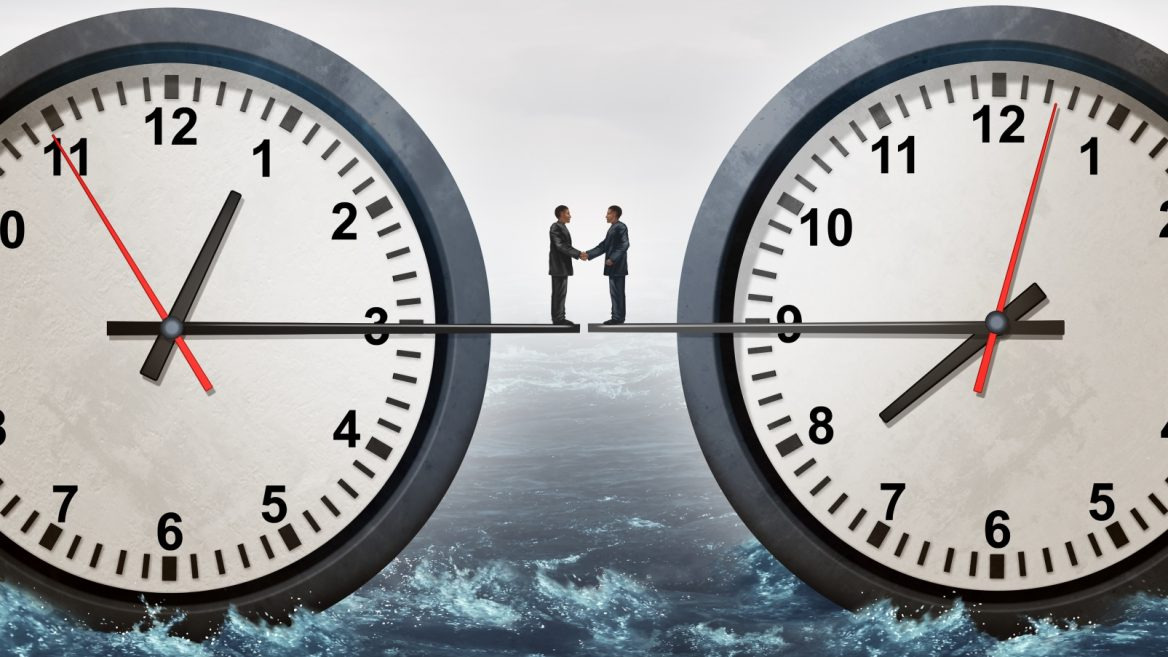
\includegraphics[width=1.0\textwidth,height=0.8\textheight]{figures/carrot.jpeg}
		\caption*{\label{fig:label} }
	  \end{figure}

	\end{column}

	\begin{column}{.43\textwidth}
	  {\footnotesize
	  Batch effect (BE) exists when:
	  \begin{itemize}
		\item Measurements from multiple subjects
		  \begin{itemize}
			  \item different patients
		  \end{itemize}
		\item Various experimental conditions
		  \begin{itemize}
			  \item treatments
		  \end{itemize}
		\item Data augmentation by combining dataset from various sources
	  \end{itemize}
	BE can be caused by various factors:
	\begin{itemize}
	  \item Instrument variation
	  \item Machine calibration
	  \item Human handling
	\end{itemize}
  }
	\end{column}
  \end{columns}
\end{frame}

% Delete this, if you do not want the table of contents to pop up at
% the beginning of each subsection:
\AtBeginSection[]
{
	\begin{frame}<beamer>{Outline}
		\tableofcontents[currentsection,currentsubsection]
	\end{frame}
}

\begin{frame}{Introduction (cont'd)}
  \vspace{-1.3cm}
  \begin{figure}[ht]
    \centering
    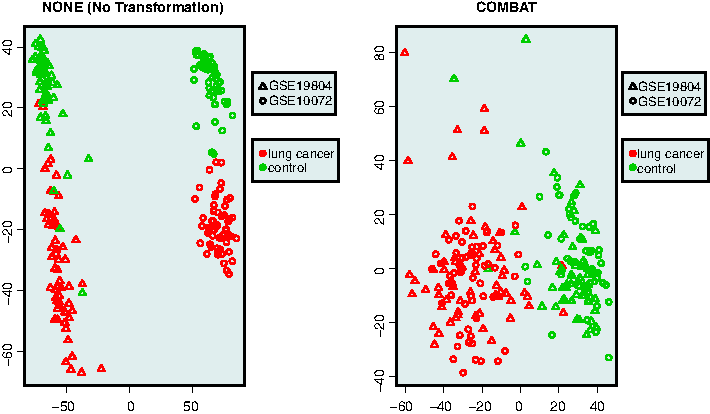
\includegraphics[width=1.0\textwidth,
    height=0.5\textheight]{figures/12859_2012_5651_MOESM2_ESM.pdf}
    \vspace{-0.7cm}
    \caption*{\tiny{\cite{Taminau2012}}\label{fig:batch-effect}}
  \end{figure}
  \vspace{-1cm}
  \begin{columns}
    \begin{column}[t]{.48\textwidth}
      \begin{itemize}
        \item Systematic errors
        \item Forming distinct groups
        \item Larger than biological variation
      \end{itemize}
    \end{column}
    \begin{column}[t]{.48\textwidth}
      \begin{itemize}
        \item Remove unwanted between-batch variations
        \item Preserve in-batch biological variability
      \end{itemize}
    \end{column}
  \end{columns}
\end{frame}

\begin{frame}{Introduction (cont'd)}
  Existing methods based on statistical modeling:
  \begin{itemize}
      \item BMC: \textbf{B}atch \textbf{M}ean \textbf{C}entered
      \parencite{Sims2008}
    \item ComBat: Location/Scale modeling with parametric/non-parametric empirical Bayes \parencite{Johnson2006}
  \end{itemize}
  \vspace{1cm}
  \begin{columns}
    \begin{column}[t]{.48\textwidth}
      Pros:
      \begin{itemize}
        \item Simple but easy to interpret
      \end{itemize}
    \end{column}
    \begin{column}[t]{.48\textwidth}
      Cons:
      \begin{itemize}
        \item Strong assumptions and constraints
          \begin{itemize}
            \item Normal distribution
            \item Similar priors
          \end{itemize}
        \item Lose biological signal
      \end{itemize}
    \end{column}
  \end{columns}
\end{frame}

\begin{frame}{Challenges}
  \begin{itemize}
    \item Difficulty in identifying real BE from measuring signal
    \item Complex data
      \begin{itemize}
        \item Non-linear
        \item Non-uniform
      \end{itemize}
    \item Unreported cause/generating factors
      \begin{itemize}
        \item Technical error
      \end{itemize}
    \item Association or correlation in various factors
      \begin{itemize}
        \item Disease
          \item Age
      \end{itemize}
  \end{itemize}
\end{frame}
\section{Methodology}
\begin{frame}{Modeling Batch Effect Using Machine Learning}
  \begin{itemize}
    \item Data-driven
    \item Powerful in modeling complex data without making strong assumption
    \item Able to learn meaningful features and denoising data
  \end{itemize}
  \begin{figure}[ht]
    \centering
    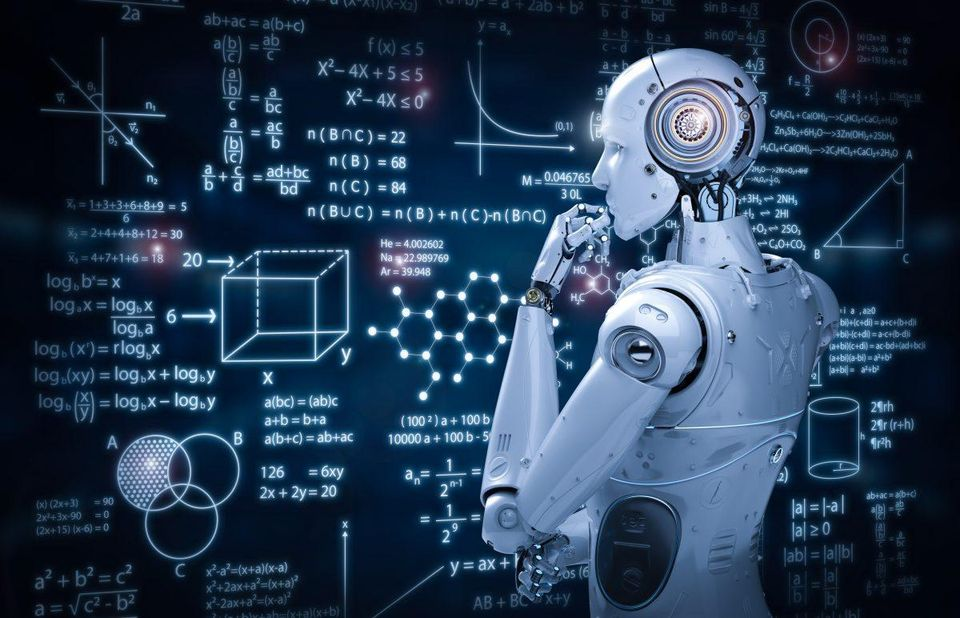
\includegraphics[width=0.5\textwidth]{figures/machine_learning.jpg}
    \caption*{\label{fig:ml}}
  \end{figure}

\end{frame}

\begin{frame}{Existing Methods Using Machine Learning}
  BE removal using autoencoder by \citeauthor*{Amodio2018} \citeyear{Amodio2018}
  \vspace{0.5cm}
  \begin{columns}
    \begin{column}[t]{.48\textwidth}
      Advantages:
      \begin{itemize}
        \item Ability to model batch effect in latent space
        \item Discriminate  the factors that are associated with batch effect
      \end{itemize}
      Disadvantages:
      \begin{itemize}
        \item Statistical alignment (percentile) of neurons distributions  one
          by one
        \item Strong assumption: batch effect in each feature is uncorrelated
      \end{itemize}
    \end{column}
    \begin{column}[t]{.48\textwidth}
      \vspace{-1cm}
      \begin{figure}[ht]
        \centering
        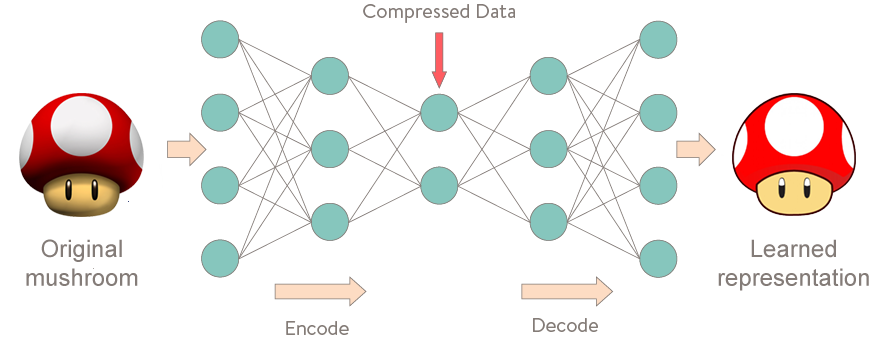
\includegraphics[width=1.0\textwidth,height=0.5\textheight,keepaspectratio]{figures/mushroom_encoder.png}
        \caption*{\vspace{0.3cm}\scalebox{0.4}{https://www.curiousily.com/posts/data-imputation-using-autoencoders/}\label{fig:be-autoencoder}}
      \end{figure}
      \vspace{-1cm}
      \begin{enumerate}
        \item Train an autoencoder to extract hidden  layer
        \item Identify batch effect related neurons
        \item Edit the neurons to correct batch effect
      \end{enumerate}
    \end{column}
  \end{columns}
\end{frame}
\begin{frame}{Existing Methods Using Machine Learning (cont'd)}
  BE removal using residual network by \citeauthor*{Shaham2017} \citeyear{Shaham2017}
  \vspace{0.5cm}
  \begin{columns}
    \begin{column}[t]{.48\textwidth}
      Advantages:
      \begin{itemize}
        \item Non-parametric
        \item More precise alignment
      \end{itemize}
      Disadvantages:
      \begin{itemize}
        \item Potential loss  of biological signal  by mapping to the entire feature space
        \item Computationally intensive
      \end{itemize}
    \end{column}
    \begin{column}[t]{.48\textwidth}
      \vspace{-1cm}
      \begin{figure}[ht]
        \centering
        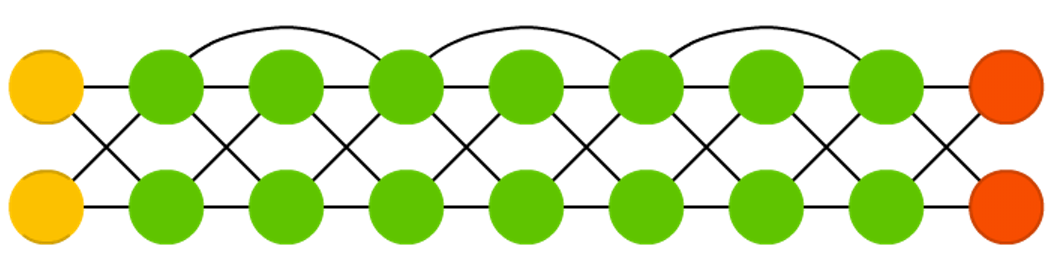
\includegraphics[width=1.0\textwidth,height=0.5\textheight,keepaspectratio]{figures/drn.png}
        \vspace*{-0.8cm}\caption*{\scalebox{0.4}{https://www.asimovinstitute.org/neural-network-zoo/}\label{fig:be-drn}}
      \end{figure}
      \begin{enumerate}
        \item Directly train the network to learn a data distribution
        \item Samples from different populations have a similar likelihood
      \end{enumerate}
    \end{column}
  \end{columns}
\end{frame}
\begin{frame}{Our Proposed Approach}
  \begin{figure}[ht]
    \centering
    \scalebox{0.9}{\input{figures/workflow.tikz}}
    \caption*{\label{fig:workflow}}
  \end{figure}
\end{frame}
\begin{frame}{Identify Batch Related Neurons}
  \begin{columns}
    \begin{column}[t]{.48\textwidth}
      \begin{figure}[ht]
        \centering
        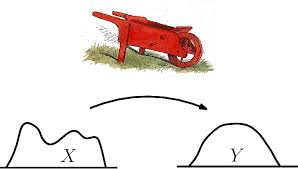
\includegraphics[width=1.0\textwidth]{figures/earth-mover-distance.jpeg}
        \caption*{\label{fig:emd}}
      \end{figure}
      \vspace{-1cm}
      Earth Mover's Distance (EMD):
      \[
        \text{EMD}(X,Y)  = \frac{\sum_{i=1}^{m} \sum_{j=1}^{n} f_{i, j} d_{i, j}}{\sum_{i=1}^{m} \sum_{j=1}^{n} f_{i, j}}
      \]
    \end{column}
    \begin{column}[t]{.48\textwidth}
      \vspace{-1cm}
      \begin{figure}[ht]
        \centering
        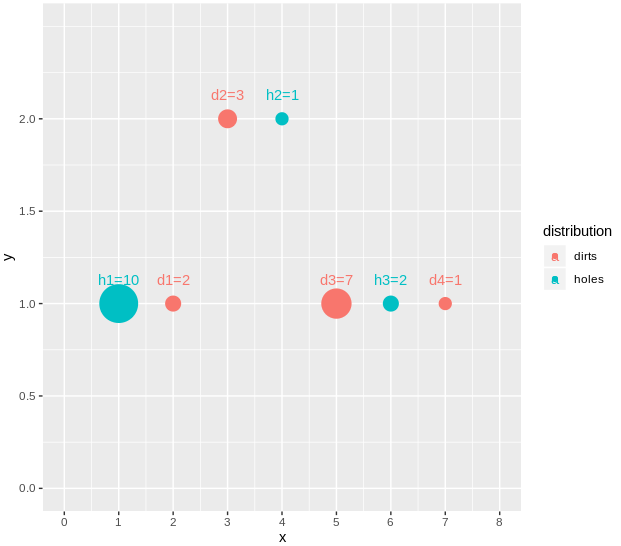
\includegraphics[width=1.0\textwidth,height=0.4\textheight]{figures/earth_points2.png}
        \caption*{\label{fig:earth-points} }
      \end{figure}
      \vspace{-1.5cm}
      \begin{table}[]
        \scalebox{0.7}{
        \begin{tabular}{lllll}
          from & to & flow & dist & work  \\
          d1   & h1 & 2    & 1.00 & 2.00  \\
          d2   & h1 & 3    & 2.24 & 6.71  \\
          d3   & h1 & 5    & 4.00 & 20.00 \\
          d3   & h2 & 1    & 1.41 & 1.41  \\
          d3   & h3 & 1    & 1.00 & 1.00  \\
          d4   & h3 & 1    & 1.00 & 1.00  \\
               &    & --   &      & --    \\
               &    & 13   &      & 32.12
        \end{tabular}
        }
      \end{table}
      EMD = 32.12 / 13 = 2.47
    \end{column}
  \end{columns}
\end{frame}
\begin{frame}{Identify Batch Related Neurons (cont'd)}
  \begin{columns}
    \begin{column}[t]{.38\textwidth}
      \begin{figure}[ht]
        \centering
        \input{figures/emd_batch_effect.tikz}
        \caption*{\label{fig:emd-batch}}
      \end{figure}
    \end{column}
    \begin{column}[t]{.58\textwidth}
      \begin{itemize}
        \item $d_{b}$: between batch EMD distance
        \item $d_{i}$: in-batch EMD distance
      \end{itemize}
      \vspace{1cm}
      \quad If any $\frac{d_{i}}{\min{(d_{b})}} < 1$:\\
      \vspace{0.3cm} \quad BE has  significant  impact in that neuron
    \end{column}
  \end{columns}
\end{frame}
\begin{frame}{Deep Learning Architectures}
  \begin{columns}
    \begin{column}[t]{.48\textwidth}
      Autoencoder:
      \begin{itemize}
        \item Layers: 54675, 512, 256, 128
        \item Activation: ReLU
      \end{itemize}\vspace{0.9cm}
      \begin{tabular}{ll}
        \toprule
        Hyperparameter&Value\\
        \midrule
        Batch size&64\\
        Learning rate&0.001\\
        Epoch&20\\
        Regularizer&$\ell_{2}$\\
        Optimizer&Adam\\
        Loss&MSE\\
        \bottomrule
      \end{tabular}
    \end{column}
    \begin{column}[t]{.48\textwidth}
      ResNet:
      \begin{itemize}
        \item 3 Blocks
        \item Activation: ReLU
      \end{itemize}\vspace{0.9cm}
      \begin{tabular}{ll}
        \toprule
        Hyperparameter&Value\\
        \midrule
        Batch size&32\\
        Initial learning rate&0.001\\
        Early stopping epoch&50\\
        Regularizer&$\ell_{2}$\\
        Optimizer&RMSPROP\\
        Loss&MMD\\
        \bottomrule
      \end{tabular}
    \end{column}
  \end{columns}
\end{frame}
\section{Results}
\begin{frame}{Dataset}
\begin{tabular}{lccccr}
  \toprule
  Dataset&Batch Number&Normal&Alzheimer&NO/AD&Total\\
  \midrule
  GSE48350&\#1&64&189&0.34&253\\
  GSE5281&\#2&74&87&0.85&161\\
  Total&2&148&276&0.54&414\\
  \bottomrule
\end{tabular}
\end{frame}
\begin{frame}{Training Autoencoder}
  \begin{columns}
    \begin{column}[t]{.48\textwidth}
      \begin{figure}[ht]
        \centering
        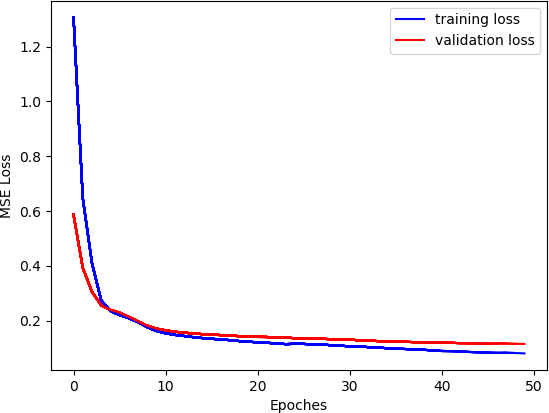
\includegraphics[width=1.0\textwidth,height=0.7\textheight]{figures/train_val_ae.png}
        \caption*{\label{fig:train-ae}}
      \end{figure}
    \end{column}
    \begin{column}[t]{.48\textwidth}
      \begin{figure}[ht]
        \centering
        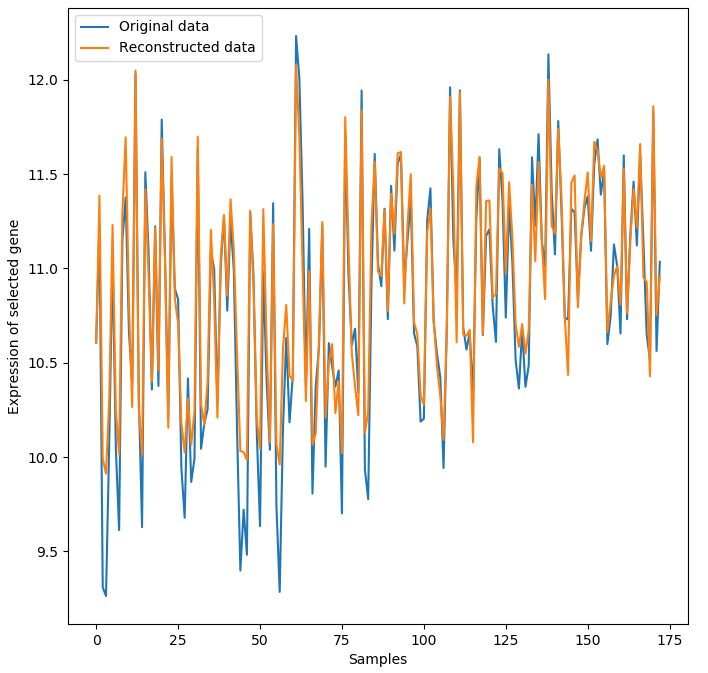
\includegraphics[width=1.0\textwidth,height=0.7\textheight]{figures/ae_reconstruction.png}
        \caption*{\label{fig:ae-reconstruction}}
      \end{figure}
    \end{column}
  \end{columns}
\end{frame}
\begin{frame}{Training ResNet}
  \begin{columns}
    \begin{column}[t]{.48\textwidth}
      \begin{figure}[ht]
        \centering
        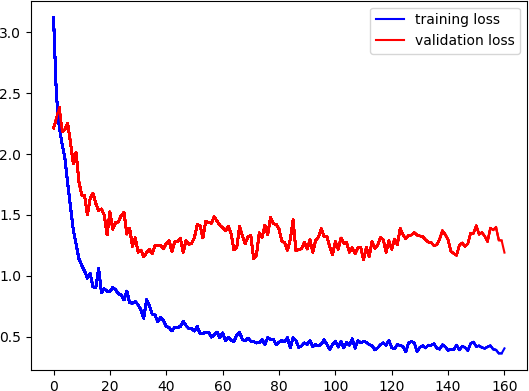
\includegraphics[width=1.0\textwidth,height=0.7\textheight]{figures/train_resnet.png}
        \caption*{\label{fig:train-resnet}}
      \end{figure}
    \end{column}
    \begin{column}[t]{.48\textwidth}
      \begin{figure}[ht]
        \centering
        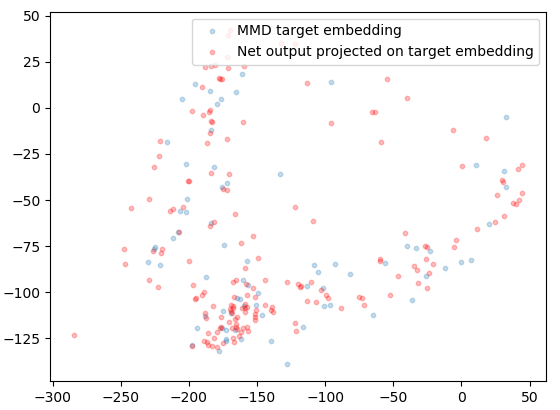
\includegraphics[width=1.0\textwidth,height=0.7\textheight]{figures/emb_resnet.png}
        \caption*{\label{fig:resnet-emb}}
      \end{figure}
    \end{column}
  \end{columns}
\end{frame}
\begin{frame}{Neurons Adjustment}
  \begin{columns}
    \begin{column}[t]{.48\textwidth}
      \begin{figure}[ht]
        \centering
        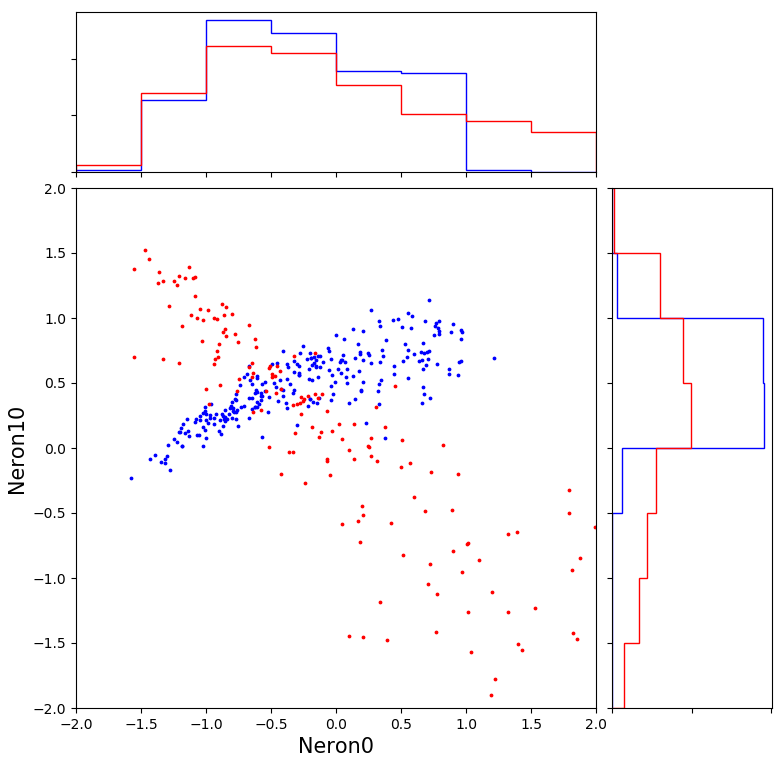
\includegraphics[width=1.0\textwidth,height=0.7\textheight]{figures/neuron_adjustment_before.png}
        \caption*{\label{fig:neuron-before}}
      \end{figure}
    \end{column}
    \begin{column}[t]{.48\textwidth}
      \begin{figure}[ht]
        \centering
        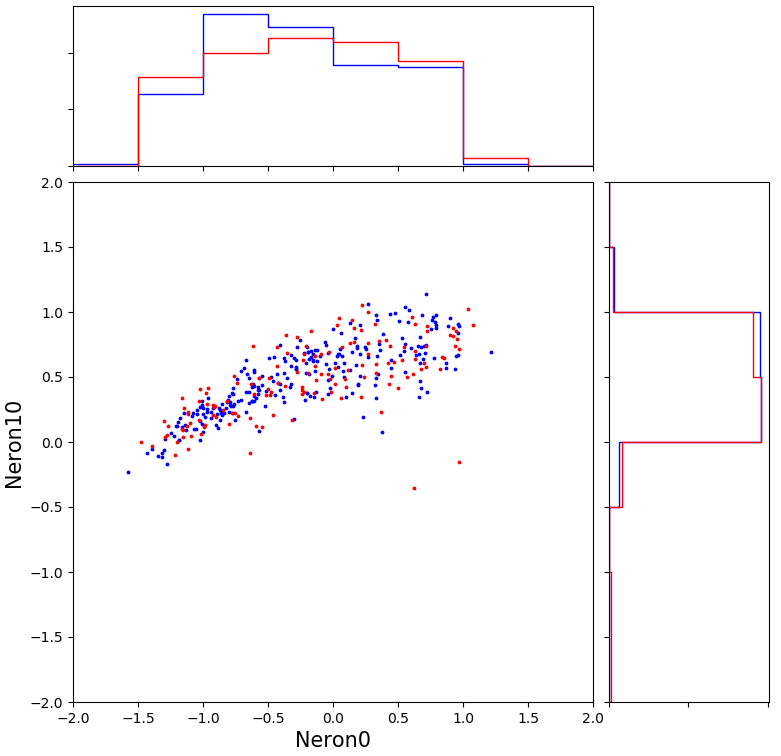
\includegraphics[width=1.0\textwidth,height=0.7\textheight]{figures/neuron_adjustment_after.png}
        \caption*{\label{fig:neuron-after}}
      \end{figure}
    \end{column}
  \end{columns}
\end{frame}
\begin{frame}{Neurons Adjustment (cont'd)}
  \begin{columns}
    \begin{column}[t]{.48\textwidth}
      \begin{figure}[ht]
        \centering
        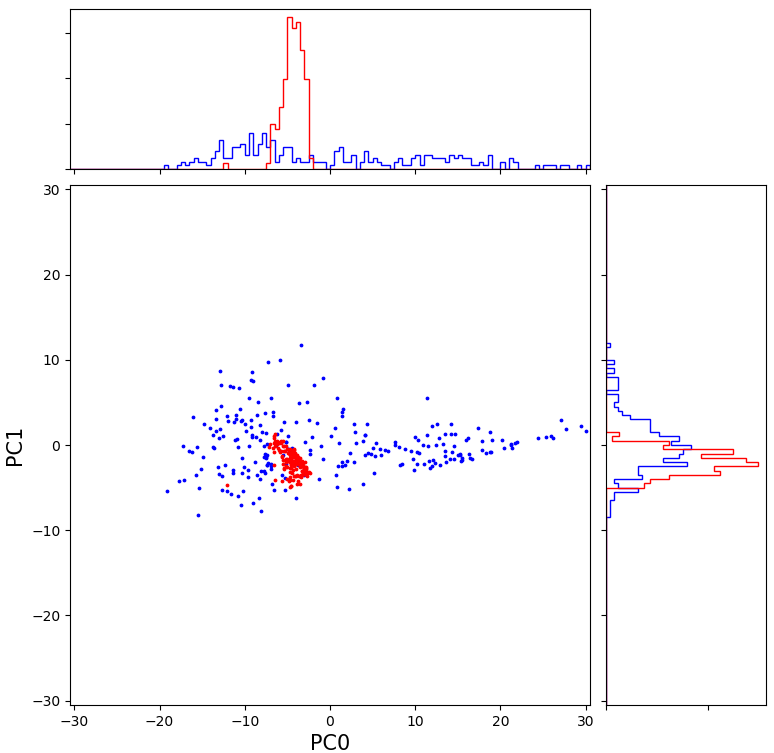
\includegraphics[width=1.0\textwidth,height=0.7\textheight]{figures/pca_before.png}
        \caption*{\label{fig:pca-before}}
      \end{figure}
    \end{column}
    \begin{column}[t]{.48\textwidth}
      \begin{figure}[ht]
        \centering
        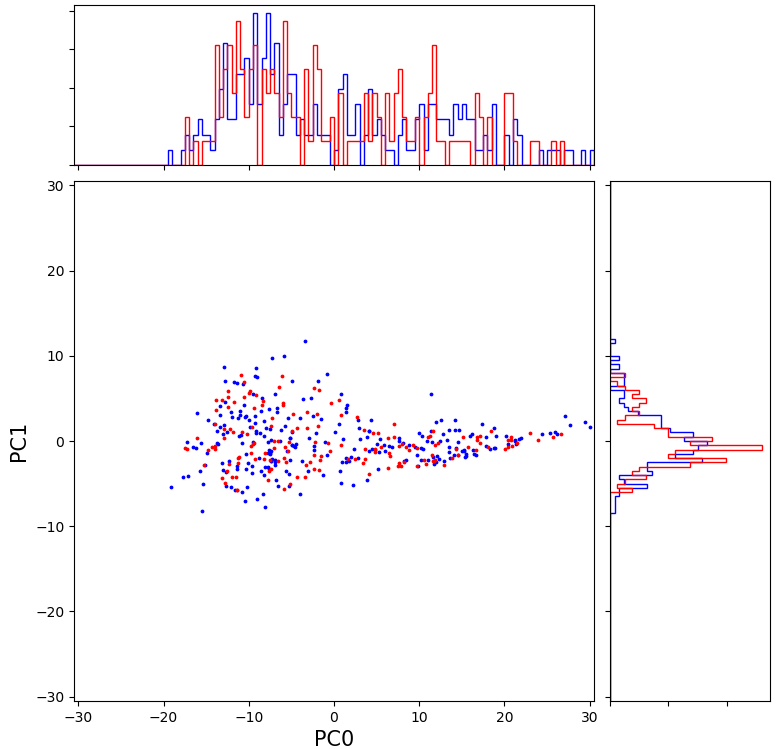
\includegraphics[width=1.0\textwidth,height=0.7\textheight]{figures/pca_after.png}
        \caption*{\label{fig:pca-after}}
      \end{figure}
    \end{column}
  \end{columns}
\end{frame}
\begin{frame}{Neurons Adjustment (cont'd)}
  \begin{columns}
    \begin{column}[t]{.48\textwidth}
      \begin{figure}[ht]
        \centering
        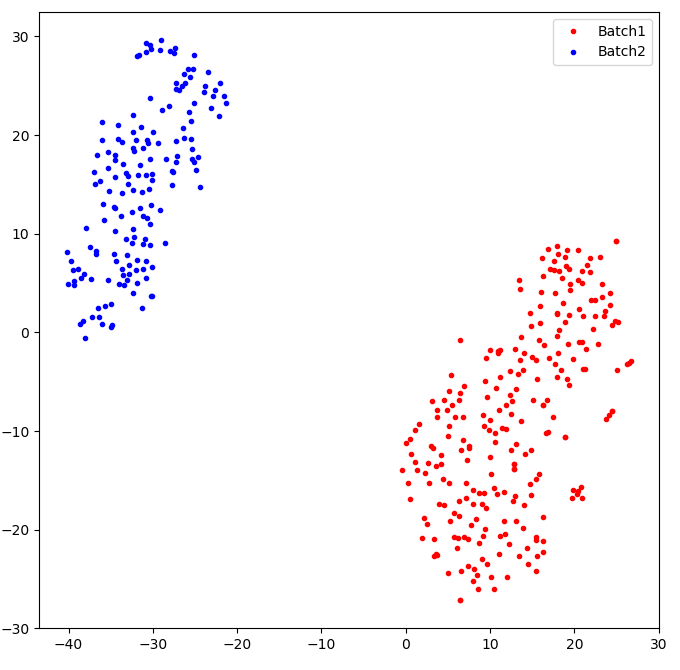
\includegraphics[width=1.0\textwidth,height=0.7\textheight]{figures/tsne_before.png}
        \caption*{\label{fig:tsne-before}}
      \end{figure}
    \end{column}
    \begin{column}[t]{.48\textwidth}
      \begin{figure}[ht]
        \centering
        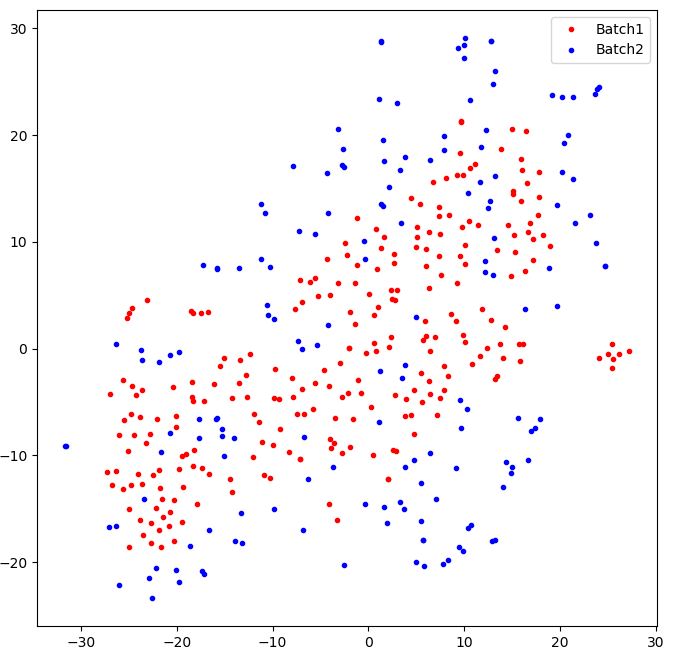
\includegraphics[width=1.0\textwidth,height=0.7\textheight]{figures/tsne_after.png}
        \caption*{\label{fig:tsne-after}}
      \end{figure}
    \end{column}
  \end{columns}
\end{frame}
\begin{frame}{Comparison}
  \begin{figure}[ht]
    \centering
    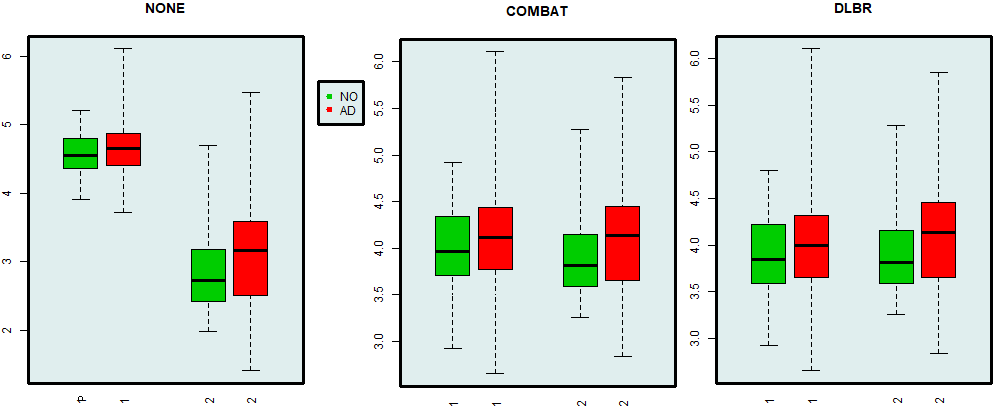
\includegraphics[height=0.4\textheight]{figures/fig7a}
    \caption*{\label{fig:7a}}
  \end{figure}
  \vspace{-1cm}
  \begin{figure}[ht]
    \centering
    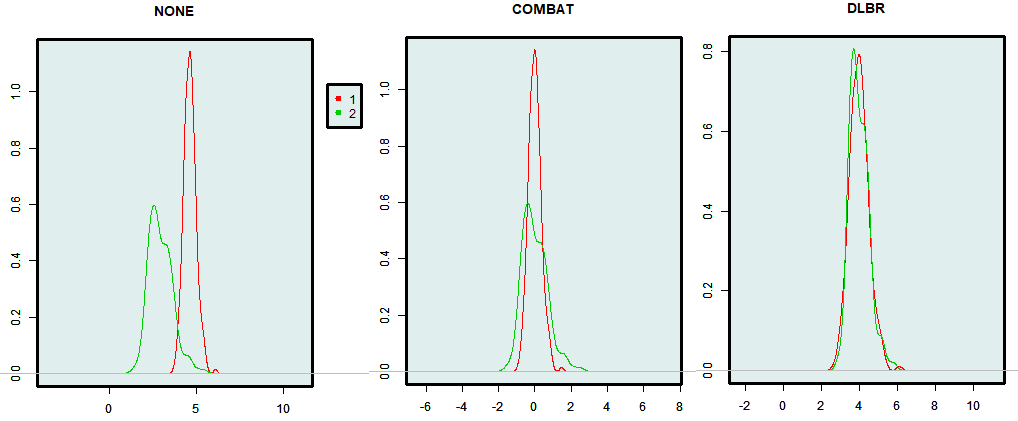
\includegraphics[height=0.4\textheight]{figures/fig7b}
    \caption*{\label{fig:7b}}
  \end{figure}
\end{frame}
\begin{frame}{Comparison (cont'd)}
  \begin{figure}[ht]
    \centering
    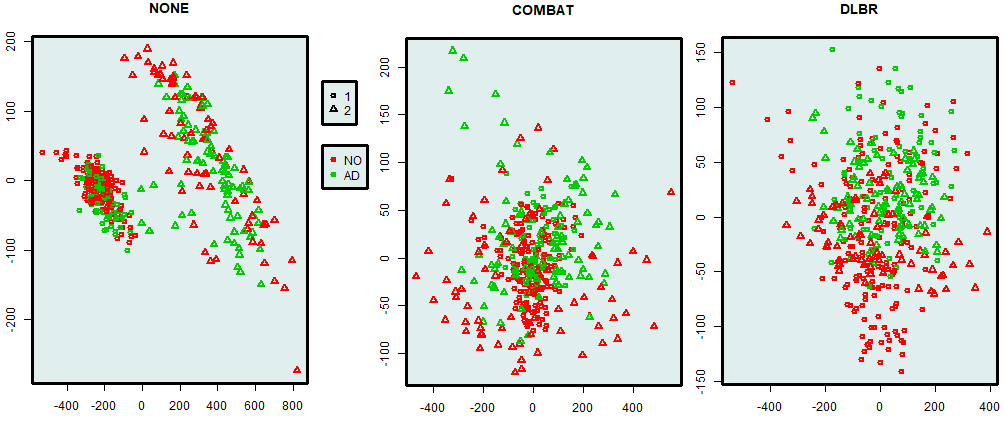
\includegraphics[width=1.0\textwidth]{figures/fig7d}
    \caption*{\label{fig:7d}}
  \end{figure}
\end{frame}
\begin{frame}{Sources of Variability Analysis}
  PCVA R package by \citeauthor*{Bushel2012} \citeyear{Bushel2012}
  \begin{figure}[ht]
    \centering
    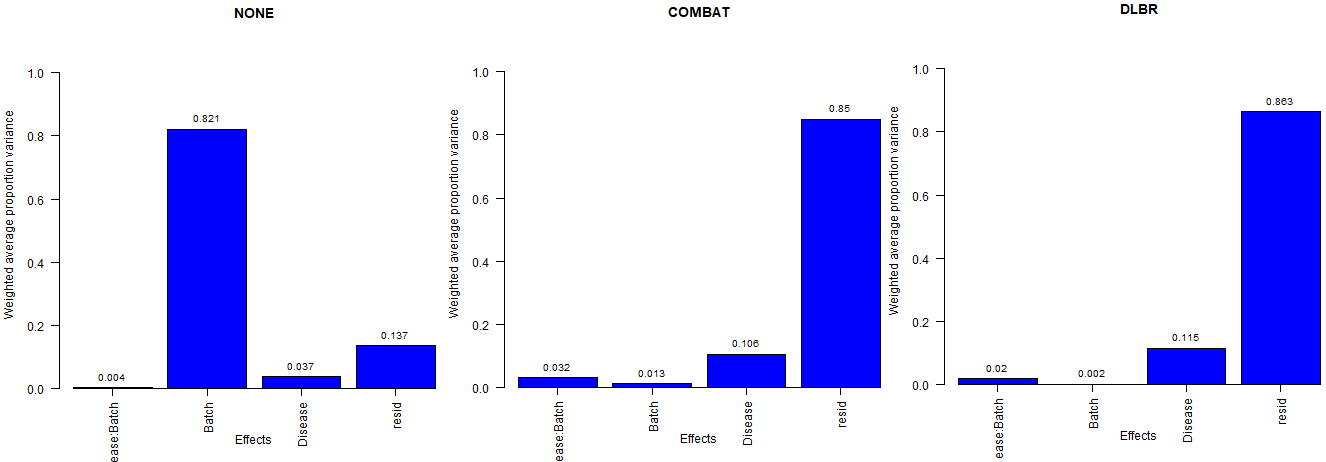
\includegraphics[width=1.0\textwidth]{figures/fig8}
    \caption*{\label{fig:fig8}}
  \end{figure}
\end{frame}
\begin{frame}{Performance Evaluation}
  \begin{columns}
    \begin{column}[t]{.48\textwidth}
      \scalebox{0.6}{
      \begin{tabular}[t]{llll}
        \toprule
        Metrics&None&COMBAT&DLBR\\
        \midrule
        Sample asymmetry\footnotemark&0.079&0.003&0.003\\
        Sample overlap\footnotemark[\value{footnote}]&340.850&248.389&225.785\\
        Samples correlation&1.000&0.918&0.924\\
        Gene overlap&0.837&0.112&0.109\\
        Gene correlation&1.000&0.967&0.982\\
        \bottomrule
      \end{tabular}
    }

    \end{column}
    \begin{column}[t]{.48\textwidth}
      \vspace{-1.7cm}
      \begin{itemize}
        \item SVM
        \item 60\% Training, 40\% Testing
      \end{itemize}
      \scalebox{0.6}{
      \begin{tabular}[t]{llll}
        \toprule
        Metrics&None&COMBAT&DLBR\\
        \midrule
        Sensitivity&0.65&0.70&0.81\\
        Specificity&0.82&0.74&0.66\\
        ACC&0.75&0.72&0.72\\
        AUC&0.73&0.72&0.73\\
        MCC&0.47&0.43&0.46\\
        \bottomrule
      \end{tabular}
      }
    \end{column}
  \end{columns}
\footnotetext{Lower is the better}
\end{frame}
\section{Conclusion}
\begin{frame}{Contributions}
  \begin{itemize}
    \item A new machine learning method  for batch effect removal
    \item Combination  of autoencoder and ResNet in modeling batch effect
    \item Dimensionality reduction and adjusting the neurons precisely
    \item Evaluate the performance on real microarray data
  \end{itemize}
\end{frame}
\begin{frame}{Acknowledgement}
  NIH-funded COBRE grant (1P20GM104320) \\
  NIH [1R01DK107264]/NIFA [2016-67001-06314]

  \begin{figure}[ht]
    \centering
    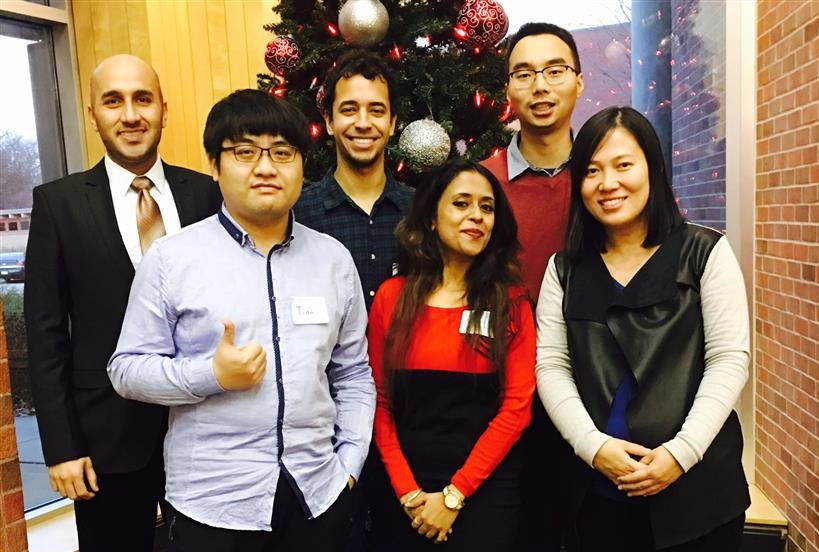
\includegraphics[width=0.7\textwidth]{figures/sbbi.jpg}
    \caption*{\label{fig:sbbi}}
  \end{figure}

\end{frame}
\begin{frame}{Questions}
	\begin{center}
		\Huge{Questions?}
	\end{center}
	\begin{figure}
		\centering
		
\includegraphics[width=0.5\textwidth, height=1.0\textheight, keepaspectratio]{figures/walter.jpg}
	\end{figure}
\end{frame}
\begin{frame}[allowframebreaks]
	\frametitle{References}
	% \bibliographystyle{chicago}
	% \bibliography{presentation}
	\printbibliography{}
\end{frame}
\end{document}

%%% Local Variables:
%%% mode: latex
%%% TeX-master: t
%%% End:
